\documentclass[a4paper,11pt,fleqn,dvipsnames,oneside,openright]{memoir} 
%\usepackage[utf8]{inputenc}
%\usepackage{graphicx}
%\usepackage{pdfpages}
%\usepackage{setspace}
%\usepackage{geometry}
\usepackage[export]{adjustbox}
\usepackage{tabu}
\usepackage{Preamble}
\usepackage{graphicx}
\usepackage[bottom]{footmisc}
\usepackage{float}

\usepackage{tocloft}
 
\setlength\cftparskip{-2pt}
\setlength\cftbeforechapskip{0pt}

\newcommand{\forceindent}{\leavevmode{\parindent=3em\indent}}

\addbibresource{references.bib} %Tilføjer kildeliste

\begin{document}

\title{
\includegraphics[width=10cm]{MujiLogo.png}}
\maketitle

\section*{Marketing - The Essentials and the Trend Drivers}

Mads Jørgsholm Bierrings\\
CPR-nr: 240793-1621\\
Business Administration and Information Systems, HA(it.) \\
5th semester\\
Examiner: Manisha Bachheti\\
Copenhagen Business School 2017/2018\\
Hand in date: 15th December 2017\\
10 Normal pages, 23.250 characters (22.450 + 800)\\

\newpage

\tableofcontents*
\addtocontents{toc}{~\vspace{-2\baselineskip}}
\thispagestyle{empty}

\mainmatter 

\chapter{Introduction}
The following chapter addresses my recommendation for the best consumer positioning in Denmark for MUJI. My analysis is based on the S-T-P\footnote{Segmentation, Targeting and Positioning} process. Throughout this chapter I will focus on the market for housewares and furniture, because I assess the markets for respectively clothes and beauty products are too competitive, thus it would be very difficult to establish a competitive advantage. %Måske komme ind på at der heller ikke er mange produkter de udbyder
MUJI has the best opportunity to establish a competitive advantage in the market for housewares and furniture. 



\section{Segmentation, targeting and positioning}
In this section I will provide an analysis based on the S-T-P process. First step is to identify the core segments. Subsequently, these segments will be analysed and compared in order to determine the size and potential of the individual segments. Next step is to select the target group expected to generate the greatest profit on the basis of an appropriate marketing mix. Finally, I will give my recommendation for the best possible consumer positioning of the company.

\chapter{Consumer positioning in Denmark}
\label{Chapter2}
\section{Introduction and delimitation}
The following chapter addresses my recommendation for the best consumer positioning in Denmark for MUJI. My analysis is based on the S-T-P\footnote{Segmentation, Targeting and Positioning} process. Throughout this chapter I will focus on the market for housewares and furniture, because I assess the markets for respectively clothes and beauty products are too competitive, thus it would be very difficult to establish a competitive advantage. %Måske komme ind på at der heller ikke er mange produkter de udbyder
MUJI has the best opportunity to establish a competitive advantage in the market for housewares and furniture. 



\section{Segmentation, targeting and positioning}
In this section I will provide an analysis based on the S-T-P process. First step is to identify the core segments. Subsequently, these segments will be analysed and compared in order to determine the size and potential of the individual segments. Next step is to select the target group expected to generate the greatest profit on the basis of an appropriate marketing mix. Finally, I will give my recommendation for the best possible consumer positioning of the company.
\subsection{Segmentation}
I have chosen to focus on three segments, because these segments represent the largest and most attractive potential target groups for MUJI. The segments I have chosen to focus on does not represent all 100\% of MUJI's customers - there might be customers younger than 18 and older than 59 years old with different preferences, but in my opinion the three segments stated below are the core segments. First of all, the segments only represent people living in Denmark, since this is the market to enter. Additionally, I only focus on the B2C market.
\newpage
The three chosen segments are:
\begin{enumerate}[label=\Alph*]
\item \textbf{Young and agnostic}\\
This segment is the young and agnostic men and women aged 18-29. This segment represent students, trainees, graduates, part-time employees and people living with their parents as well as the people with their own homes.
\item \textbf{Settled middle youth}\\
This segment is the middle youth men and women aged 30-44. This segment represents the full-time employees, parents of young children, owners of detached houses, vehicle owners and settled families.
\item \textbf{Hard working mid-lifers}\\ 
This segment is the mid-lifers aged 45-59. This segment represents people who work a lot and have been on the labour market for a long time, and parents whose children have become young adults and might have left home.  
\end{enumerate}




\subsection{Targeting (SOCC analysis)}
\subsubsection{Analysis and comparison of segments}
In the following section, I will analyse and evaluate the three segments by using the SOCC\footnote{Size, Opportunities, Cost, Competition} analysis. In the analysis I will compare different criteria such as \textit{age}, \textit{size}, \textit{growth}, \textit{proportion and expected future proportion in the overall market}, \textit{type of dwelling} (geographic spread), \textit{income} etc.

\begin{table}[H]
\centering
\caption{Comparison of size of segments in year 2013 - 2014 \cite[15-18]{ConsumerLifestyles}}
\label{SegmentsTable}
\begin{tabular}{l|llll}
\textbf{Segment}        & \textbf{A}   & \textbf{B}     & \textbf{C}    &  \\ \cline{1-5}
Age                         & 18-29   & 30-44     & 45-59     &  \\
Size                        & 847.900 & 1.073.000 & 1.159.000 &  \\
Growth                      & 2,5\%   & -1,5\%    & 0,35\%    &  \\
Proportion in the market    & 15,1\%  & 19,1\%    & 20,6\%    &  \\
Expected proportion in 2020 & 15,7\%  & 17,7\%    & 20,6\%    & 
\end{tabular}
\end{table}

\textbf{Size, growth and proportion of the overall market from year 2013 - 2014.}
As shown in table \ref{SegmentsTable}, the segment with the greatest amount of people is segment C, with a population of 1.159.000 people and a growth rate of 0,35\%. The smallest, but also the fastest growing segment, is segment A with a population of 847.900 people and a growth rate of 2,5\%. The population of segment B was 1.073.000 people and the growth rate was negative with -1,5\%. These trends are expected to continue in the next couple of years, and the difference in the overall proportion for segment A and B are expected to converge even more, which makes segment A quite attractive. A factor that might have a negative effect on the purchasing power of segment A, is that 41\% of people aged 18-25 live with their parents, and only 28\% of people aged 25-29 had their own home in 2014 \cite[12]{ConsumerLifestyles}.
\\\\
\textbf{Residents and income.} As we can see in appendix \ref{ResidentsAge}, segment A represents the largest proportion of people living in apartments. With this I assume that segment A is the segment with the largest proportion of people living in urban areas. Segment B and C represent the largest proportion of people living in detached houses and linked or semi-detached houses, which makes sense, because people in these segments might have children and cars. With this I assume that segment B and C are the segments with the largest proportion of people living in rural areas. These factors have great influence on how the marketing mix should be put together. \par

\forceindent As we can see in table \ref{DisposableIncomeTable}, segment C certainly has the largest proportion of income and the highest average monthly income. This is not necessarily positive because it might indicate that the segment will buy more expensive products than the products MUJI sells. Segment B has the second highest amount of income as well as average, monthly income, but this segment represents people, who on average have more expenses compared to segment A and C, because of children, cars etc. 

\begin{table}[H]
\centering
\caption{Income year 2016 based on appendix \ref{DisposableIncome}}
\label{DisposableIncomeTable}
\begin{tabular}{lllllll}
\multicolumn{1}{l|}{\textbf{Segment}}         & \textbf{A}      & \textbf{B}      & \textbf{C}      &  &  &  \\ \cline{1-4}
\multicolumn{1}{l|}{Amount of income (1.000)} & 100.392.471 kr. & 274.959.609 kr. & 347.929.813 kr. &  &  &  \\
\multicolumn{1}{l|}{Average monthly income}   & 11.573 kr.      & 21.926 kr.      & 24.818 kr.      &  &  &  
\end{tabular}
\end{table}

\textbf{Opportunities of influencing the target group and cost needed in order to confront the segment.} The people in segment A are using Facebook less frequently than before, but Snapchat and Instagram are very popular in this segment \cite[13]{ConsumerLifestyles}. Instagram is especially a good place for branding and inspiration, and can be used to target the segment with more authentic and relatable marketing material, eventually posted by customers \cite{GetReal}. Another obvious place to meet this segment is at the educational institutions. Segment B is highly active on social media with 74\% of consumers aged 35-44 having a presence on social media sites \cite[15]{ConsumerLifestyles}. Facebook and LinkedIn are potential channels to reach this segment, but those channels are not the best channels in terms of inspiring the consumers, because consumers generally use other channels to get inspired. Segment C is less active on social media than the other two segments. This segment focuses more on work and many people in this group work for more than 45 hours a week. This segment, taken the products and philosophy of MUJI into consideration, is more difficult and more expensive to influence compared to segment A and B, who are more present on the channels apposite for inspirational advertising. Social media is one of the best and cheapest ways to confront a target group, and it is optimally to confront the segment with marketing material as authentic and relatable as possible. 
\\\\
\textbf{Competition.} The segment with the least intensive competition is segment A, because I believe there is a gap in the market, missing a low- to mid-priced brand with high quality and minimalist furniture and housewares. This aspect is elaborated in chapter \ref{CompetitionPorters}.


\subsubsection{Choice of target group}
Based on previous analysis, my recommendation for the best possible target group is \textbf{segment A; Young and agnostic}. This is the fastest growing segment, the price- and quality-oriented students and graduates, who are curious, inspiration seeking and agnostic shoppers, who cannot be fooled with labels \cite{Top10Trends}. This segment is not representing the highest amount of income, nor has it the greatest size, but it is definitely the segment where MUJI has the opportunity to provide an excellent marketing mix and establish a competitive advantage. The choice of this target group also supplements the opinion of the Executive of Muji - "We have to get younger customers" - Kei Suzuku \cite{FutureGrowth}.

\subsection{Positioning (The 4 P's)}
Figure \ref{PositioningMap} on the next page shows my recommendation for the best consumer positioning for MUJI in relation to the target group. I will use the 4 P's\footnote{Product, Place, Promotion, Price} in the following section to quickly outline how MUJI should define their marketing mix in order to differentiate themselves from the competitors.  
\\\\
\textbf{Product}. Simple, functional, minimalist and good quality products with no labels, meeting the demands of the young agnostic shoppers. 

\textbf{Price}. Low- to mid-price. This parameter is elaborated in chapter \ref{Chapter3}.

\textbf{Place (distribution)}. Bricks and mortar shop in Copenhagen. Furthermore, the webshop should be prioritised highly, because of the increase in consumer expenditure online. From 2014 - 2018 online sales are expected to increase with 27,7\% in Denmark \cite[5]{ConsumerLifestyles}. 

\textbf{Promotion}. Authenthic, inspirational and not-pushy campaigns and material reaching the target group through social media, story telling and exhibitions. 

\begin{figure}[H]
    \centering
    \caption{Positioning map (\ref{Competitors})}
    \label{PositioningMap}
    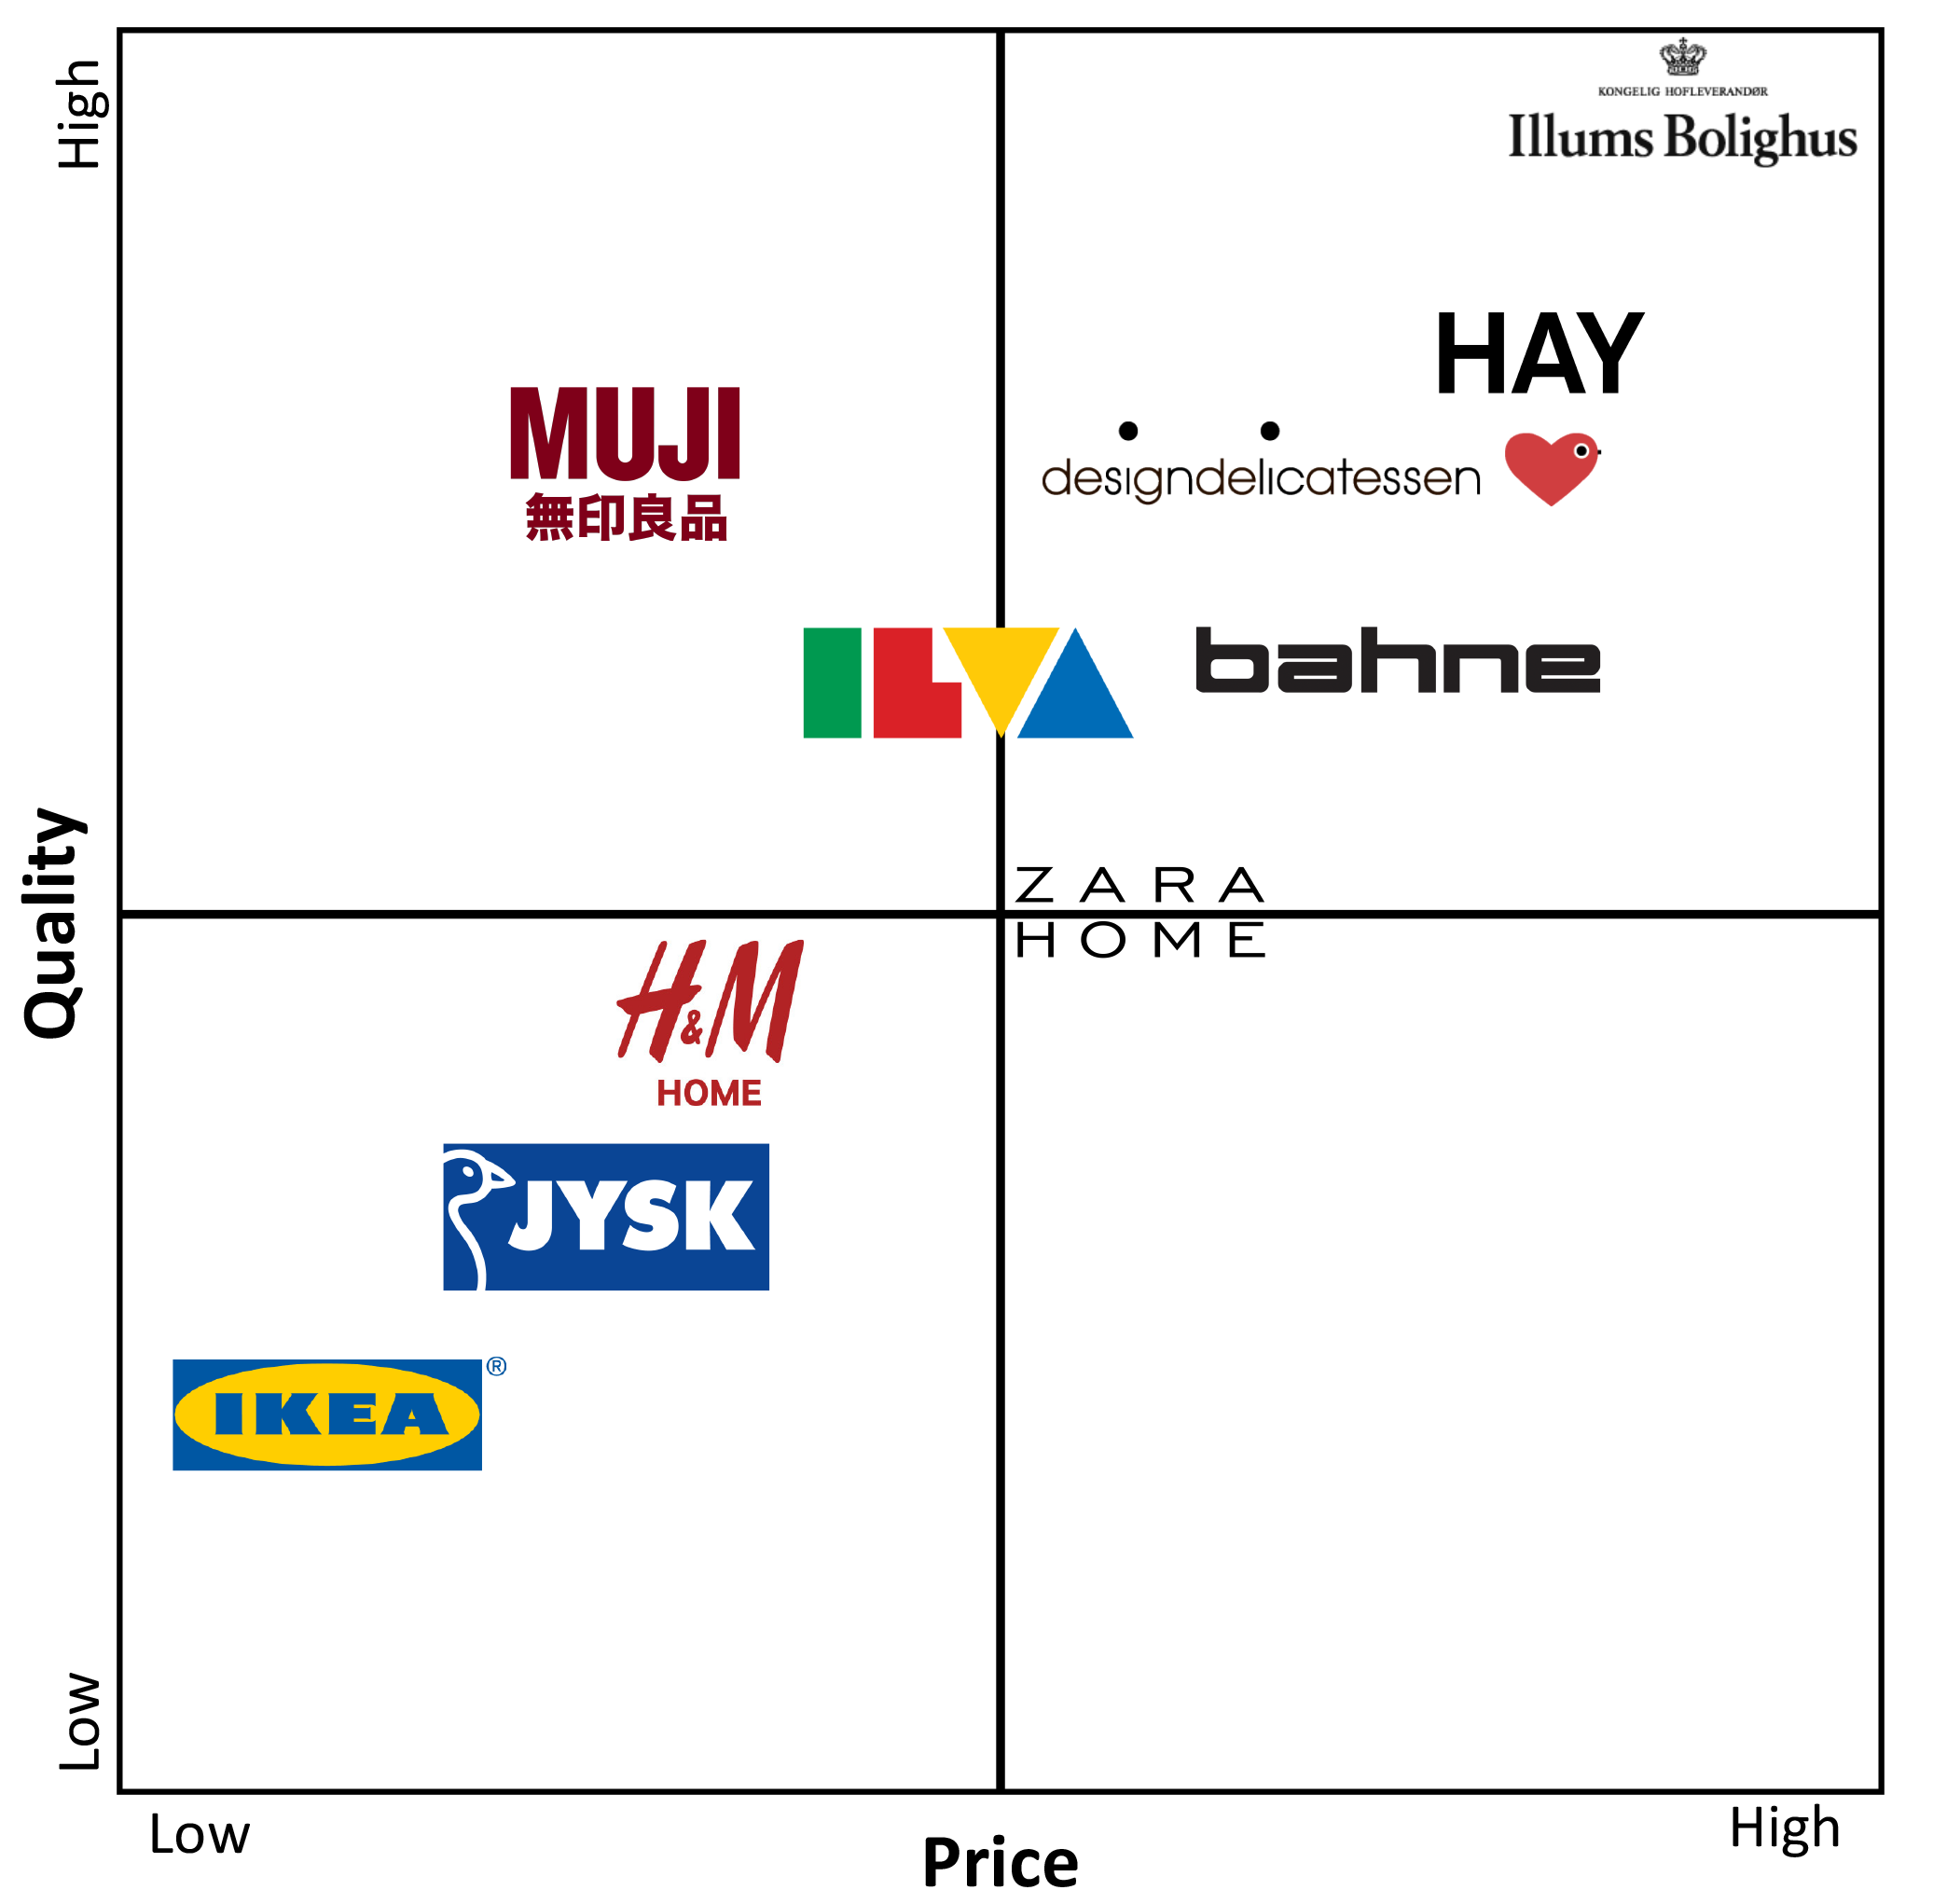
\includegraphics[width=12 cm]{ConsumerPositioning/CompetitionMapV3.png}
\end{figure}


\section{Summary}
In this chapter, I have conducted an analysis in order to recommend the best possible consumer positioning for MUJI in Denmark. Firstly I have identified the core segments, where after I have evaluated and compared each of these segments using the SOCC approach. Based on the analysis I have chosen a target group and finally drawn together the optimum marketing mix to confront this group. The result of my analysis is illustrated in figure \ref{PositioningMap} above. The approach I have had to the challenge is just one of many ways to approach it. Another approach could be to use Porters 5 Forces, the BCG model, 4 C's and so fourth. I think the most important aspect in this matter is to always keep the needs of the customer in focus, which my approach most certainly does. 


\chapter{Pricing strategy}
\label{Chapter3}
\section{Introduction and delimitation}
In this chapter, I will present my proposal as to which pricing strategy MUJI should use. In order to choose the right strategy, I will conduct an analysis of the market by using Porters 5 Forces. Based on the analysis, I will then determine which strategy MUJI should use to gain an competitive advantage. As in previous chapter, I will focus on the market for homewares and furniture. 
\section{Porters 5 Forces}
The purpose of using Porters 5 Forces is to gain an understanding of the market, including MUJI's position in relation to \textit{new entrants}, \textit{suppliers}, \textit{substitutes}, \textit{customers} and \textit{competitors}.

\subsubsection{Threat of new entrants}
The threat of new entrants in the market for housewares and furniture exists but is not very dominant, because of barriers in terms of economies of scale and high initial investments. The existing players on the market are quite large and have many advantages in relation to cost and production, and potential new entrants would have to invest heavily in order to compete on price and quality.

\subsubsection{Bargaining power of suppliers}
MUJI's bargaining power in relation to the suppliers is high, because of their size and growth. MUJI's revenue was more than 307 million yen in FY2015 with an operating profit of 34,4 million yen, representing an increase of 18,2\% of revenue and 44,4\% of profit \cite[2]{Annual}. This shows that MUJI is growing fast and therefore is becoming an even larger customer for the suppliers.     

\subsubsection{Threat of substitutes}
The threat of substitutes is one of the most important forces to consider, since the consumers in Denmark has become a nation of bargain hunters \cite[35]{ConsumerLifestyles}. An opportunity for MUJI to influence the power of substitutes, is that the danish consumers are getting ready to prioritise quality over price again \cite[35]{ConsumerLifestyles}, which gives rise for an appropriate marketing mix. 

\subsubsection{Bargaining power of customers}
MUJI's bargaining power in relation to the customers is low, because of the many alternatives in the market provided by the competitors. The market has a high elasticity, and therefore it is very important for MUJI to differentiate themselves from their competitors in order to minimise the bargaining power of the customers.

\subsubsection{Competitive rivalry between existing players}
\label{CompetitionPorters}
The competitive rivalry between existing players on the market is high. There are many companies of about the same size and much competition on price. For example in the low-price category where IKEA, Daells Bolighus, Biva etc. are located, there is an intensive competition on price. Likewise there are many high-price companies such as Illums Bolighus, HAY, Designdelicatessen and Ilva competing on brand, design and quality. A third region in the market, consists of smaller companies selling high qualiy products with less focus on brand value. The problem for these companies, is the fact that they do not have advantages in terms of economies of scale, which is why the products are expensive. This is the opportunity for MUJI, because they have advantages in terms of economies of scale and additionally they do not seek high brand value. 


\section{Pricing strategy}
Based on the the conclusion from chapter \ref{Chapter2} regarding the consumer positioning, and the considerations from the analysis in previous section, we can now determine the pricing strategy.  

\subsection{Criteria for a successful pricing strategy}
The pricing strategy needs to be adapted by the chosen target group; Young and agnostic. Furthermore we need to respect MUJI's philosophy about high quality products and fair prices \cite{FutureGrowth}. Other than that, we might as well select a pricing strategy with respect to the Executive's plan of making prices that only varies with a maximum of 30\% globally \cite{FutureGrowth}. Finally, MUJI needs to differentiate themselves from the competitors. 

\subsection{Perceived value pricing}
My proposal as to which pricing strategy MUJI should use in order to meet the criteria stated above, is the perceived value pricing, more specifically with a high-value strategy. The consumers in the chosen target group are not interested in products with labels and high brand value, they are looking for bargains and quality. One of the biggest global consumer trends for 2016 was that consumers are finding quality in unknown, unadvertised brands, which fits well with MUJI's concept of no brand. This pricing strategy is a good opportunity for MUJI to differentiate themselves from the competitors, offering minimalist quality products at fair prices. Today, the alternative for buying cheap products from IKEA or the like, is to buy overpriced products from high-brand companies. There seem to be a gap in the market covering the need for the consumers who wish to buy products exclusively for the quality, and not for the brand or image. My proposal is consistent with my recommendation in previous chapter illustrated with a positioning map, figure \ref{PositioningMap}. This gap is where MUJI wants to be.  
\section{Summary}
In this chapter, I have concerned the market using Porters 5 Forces in order to support the pricing strategy of my proposal. One might argue that Porters 5 Forces is no longer viable and not comprehensive enough to predict the market dynamics of today, which are affected by technology, disruption and globalisation. With that said, I think it gives a picture of the market, and I certainly think it supports my final choice of pricing strategy. The pricing strategy I found to be the best for MUJI is the perceived value pricing.  

\chapter{Future trends}
\section{Introduction}
In this chapter, I will provide my recommendation as to which future trends MUJI must be aware of in relation to its commercialisation, and how they should act on these trends. 
\section{Trends}
\subsubsection{Consumer expenditure on the internet}
This is one of the most important trends to be aware of and act upon, as the internet retailing continues to show record growth. The internet retailing has more than doubled in the years from 2009 - 2014\footnote{Euromonitor: Consumer lifestyles in Denmark}. This trend is expected to continue to increase and therefore it is very important for MUJI to prioritise their presence online, the webshop and the visual identity of the company.  

\subsubsection{Tea is the future}
According to Euromonitor, tea, and especially japanese and chinese green tea, is the new coffee for danes \cite[29]{ConsumerLifestyles}. MUJI tea is apparently not available in EU or US according to the associated webshops, but the webshop for MUJI in Hong Kong\footnote{https://www.muji.com.hk/en/sub-category.php?dept=123&id=113&c=005} sell it. I think this trend is an obvious opportunity for MUJI to attract more consumers. My recommendation in order to take advantage of this trend, is to open an in-store cafe offering a variety of tea when the shop in Copenhagen is launched.  

\subsubsection{Agnostic shoppers}
This trend is one of the reasons for my choice of positioning and pricing strategy. The agnostic shoppers are not only the young people, but I think, however, they make up for the majority. They are intrigued by innovation around value \cite[3]{Top10Trends}, which opens up another opportunity for MUJI. MUJI designers came up with a bath towel that has a next life, which can be used as a bath math, and finally, as a duster \cite{FutureGrowth}. This kind of innovative products is the essence of innovation around value, and MUJI should continue to play around with new use of traditional products.   

\subsubsection{Changemakers}
The last trend I recommend MUJI to be aware of, and to act upon, is the "Changemakers". Social causes and climate change gets more attention, and companies as well as individuals are more concerned about these problems \cite[14-17]{Top10Trends}. This trend can also be used to establish a competitive advantage. I do not have the impression that sustainability is an essential element for MUJI, but I recommend MUJI to spend more effort in this regard and focus on sustainability and CSR, in relation to the products as well as the advertising. According to the Executive, MUJI has a good relationship with the suppliers and they care about them\cite{FutureGrowth}, which I think should be a part of their identity.

\chapter{Cultural aspects}
\section{Introduction}
In this chapter, I will present my recommendation on how MUJI should consider and act concerning cultural aspects of working in Denmark. Furthermore, I will enlighten what impact culture may have on advertising. 
\section{Cultural aspects of working in Denmark}
My recommendation as to which cultural aspects of working in Denmark MUJI should consider and act upon, is presented with a comparison of the difference between Denmark and Japan on various aspects. The differences are also illustrated in appendix \ref{CultureComparison}. 

\subsubsection{Hierarchy and status}
The hierarchy in Japan is very steep compared to Denmark. In Denmark we are actually opponents to steep hierarchies, because we believe that the bureaucracy belongs to the past. In Denmark we strive to be as agile as possible, and to allocate decision rights to the individuals in the various departments. Compared to the culture in Japan we have a very informal culture regarding status
and we do not consider age as a measure of status for example, which is the case in Japan \cite{JapaneseCulture}. 

\subsubsection{Deal or relationship focus}
Relationship before business is a very important aspect of doing business in Japan. In Denmark we are more straightforward and we prioritise to focus on business over relationship.  

\subsubsection{Trust, conflicts and communication}
In Japan trust is something to be gained and no business will be discussed until a relationship between the stakeholders has been established. In Denmark we actually, as default, have trust in strangers until it eventually is devastated. In Japan and Asia, in general, conflicts are to be avoided in order to maintain face. In Denmark we believe it is important to face and solve any potential conflicts. The culture in Japan concerning communication is very indirect, and direct communication is seen as impolite and crude. In Denmark we have a very direct way of communicating, and we consider direct and honest sayings to be respectful and efficient \cite{Communication}.    

\subsubsection{Time and group vs. individual}
In Denmark we are very strict concerning time, and we believe that deadlines and agreements must be respected. In Japan there is a more relaxed attitude to deadlines and agreements. In Denmark the individual takes priority, and in Japan the group takes priority. These aspects are very important to consider because they have great influence on the motivation of the employees. 

\section{Cultural impact on advertising}
The culture also has great impact in regard to advertising. The global consumer, as a concept, is overrated\footnote{Session 8 slidepack, slide 58}, and the advertising must be adapted locally to the individual country. One of the most important aspects to consider regarding advertising is weather to use a hard sell or soft sell strategy \cite{Sell}. In Japan a soft sell strategy for advertising is most appropriate, whereas a hard sell strategy definitely is more appropriate in Denmark. The hard sell strategy is my recommendation for MUJI to use. The people in Denmark are, as described above, more direct and straightforward and the advertisement has to appeal to the individual determinism. Furthermore, a hard sell strategy is obvious is order to confront the target group recommended in chapter \ref{Chapter2}.  

\chapter{Conclusion}
In this report, I have analysed, evaluated and compared various aspects to a variety of challenges, in order to specify my recommendations to be discussed at the management meeting next week. The consumer confidence in Denmark is at the highest level since 2006, and the population is getting ready to prioritise quality over price again \cite{ConsumerLifestyles}. This is just one of many aspects indicating the attractiveness of the danish market. The competition is tough, but I have identified a gap in the market, which represents an opportunity for MUJI's entry.
\\\\
Considering my recommendations regarding consumer positioning, pricing strategy, future trends and cultural aspects, my final advice for MUJI is to proceed and enter the danish market. I am very certain that MUJI will become a success, and they will be able to establish a competitive advantage. This advice only applies with my recommendations as a prerequisite.




% Kildeliste - brug \cite{} ved henvisning
\begingroup
	\raggedright
	\printbibliography
\endgroup 

% Bilag - brug \ref{} ved henvisning
\appendix
\chapter{Appendix}
\numberwithin{equation}{section}

\section{Competitors}
\label{Competitors}
List of competitors:

\begin{itemize}
    \item
    Zara Home
    \\
    \url{https://www.zarahome.com/dk}
    \item
    H\&M Home
    \\
    \url{http://www2.hm.com/da_dk/home.html}
    \item
    IKEA
    \\
    \url{http://www.ikea.com/dk/da/}
    \item
    Bahne
    \\
    \url{https://www.bahne.dk/}
    \item
    Ellos
    \\
    \url{https://www.ellos.dk/}
    \item
    Imerco
    \\
    \url{https://www.imerco.dk/}
    \item
    Kop\&Kande
    \\
    \url{https://www.kop-kande.dk/}        
    \item
    Illums Bolighus
    \\
    \url{https://www.illumsbolighus.dk/}  
    \item
    HAY
    \\
    \url{http://hay.dk/da-dk} 
    \item
    JYSK
    \\
    \url{https://jysk.dk/}
    \item
    Designdelicatessen
    \\
    \url{https://designdelicatessen.dk/} 
\end{itemize}

\section{Residents by age in Denmark}
\label{ResidentsAge}
The numbers in this statistic is from year 2017 and comes from the table BOL201 from Statistics Denmark \cite{DanmarksStatistik}. 

\begin{center}

\includegraphics[width=10cm]{Appendix/Residents.png}
\end{center}

\newpage 

\section{Disposable income for people living in Denmark}
\label{DisposableIncome}
The numbers in the table are based on statistics from Statistics Denmark. The specific statistic used for the table below is table: INDKP106. \cite{DanmarksStatistik} 

\begin{center}

\includegraphics[width=14cm]{Appendix/DisposableIncomeTotal.png}
\end{center}

\textbf{Total income for segment A, B and C:}


\begin{equation}
Young\:and\:ambitious = 40.139.911+60.252.560=100.392.471kr.
\label{YoungIncome}
\end{equation}
\label{MiddleIncome}
\begin{equation}
Midddle\:youth = 72.337.548+89.777.735+112.844.326=274.959.609kr.
\end{equation}
\label{MidIncome}
\begin{equation}
Mid\:lifers = 118.769.188+124.808.024+104.352.601=347.929.813kr. 
\end{equation}

\textbf{Average monthly income for segment A, B and C:}

\label{YoungIncomeAverage}
\begin{equation}
Young\:and\:ambitious =
\frac{(9.009+14.137)}{2}=11.573 kr.
\end{equation}
\label{MiddleIncomeAverage}
\begin{equation}
Midddle\:youth =
\frac{(18.925+22.281+24.572)}{3}=21.926 kr.
\end{equation}
\label{MiddleIncomeAverage}
\begin{equation}
Mid\:lifers =
\frac{(25.375+24.950+24118)}{3}=24.818 kr.
\end{equation}

\section{The business culture in Japan vs. in Denmark}
\label{CultureComparison}


\begin{figure}[H]
    \centering
    \caption{Comparison of Japan and Denmark}
    
\includegraphics[width=12cm]{Appendix/CultureTable.png}
    \label{fig:my_label}
\end{figure}


\end{document}
